% Generated by thesis/ch7/exp1/make_figures.py -- do not edit by hand.
\begin{figure}[tbp]
  \centering
  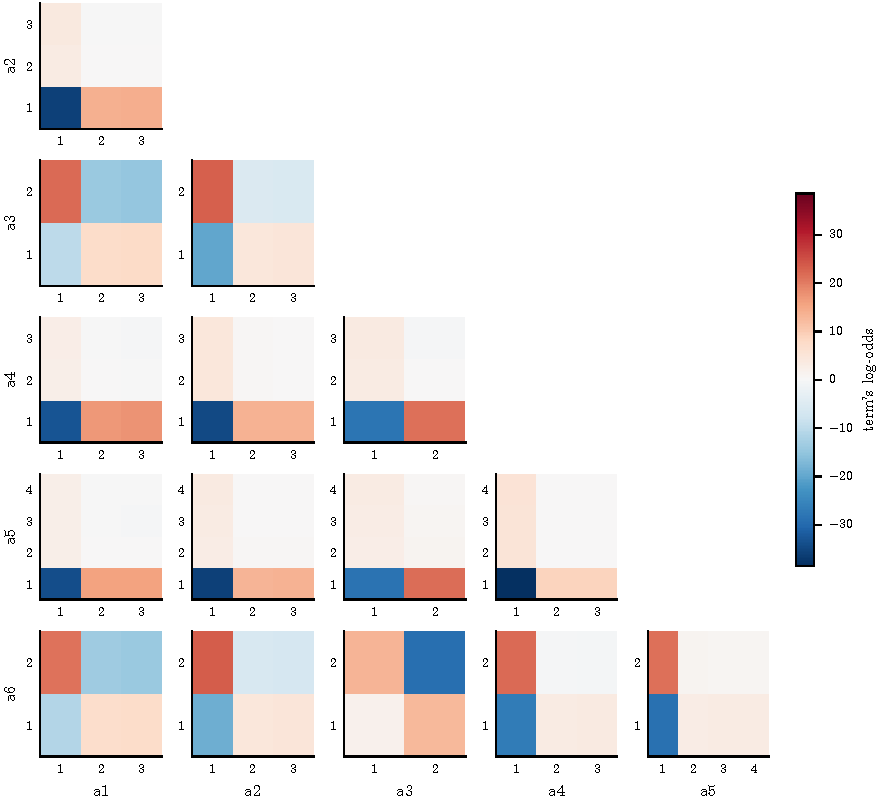
\includegraphics[width=\textwidth,height=0.8\textheight,keepaspectratio]{figures/ch7/ebm-monk2-pairs.pdf}
  \caption{MONK-2: the 15 pairwise terms of the explainable boosting machine on the six raw attributes. One panel per pair of attributes $a_i$ (across) and $a_j$ (up), each axis the attribute's values, value 1 (the first value) at the lower left; colour: the term's log-odds (red raises, blue lowers), one scale for all panels.}
  \label{fig:ch7-ebm-monk2-pairs}
\end{figure}
